% Chapter 5

\chapter{État de l'art de la récupération du flux vidéo} % Main chapter title

\label{Chapter5} % For referencing the chapter elsewhere, use \ref{Chapter5} 

%----------------------------------------------------------------------------------------

\section{Webcam USB}

Afin de mieux comprendre l’utilisation de Video4Linux nous avons effectué plus de
recherches sur celui-ci et nous sommes tombés sur un blog expliquant la récupération d’un
flux vidéo d’une webcam USB avec V4L2 sur imx6. Nous avons donc essayé de capturer le flux
de notre webcam USB dans un premier temps, une fois ceci fonctionnel nous passerons sur le
flux vidéo de la Raspi Cam v2. Nous avons récupéré une webcam USB afin de tester les
différentes commandes proposées par le blog et essayer de capturer le retour vidéo.

Dans un premier temps il est nécessaire de récupérer sur quel port est connecté la
webcam USB, pour cela on utilise la commande : \textbf{lsusb -t}

\begin{figure}[th]
    \centering
    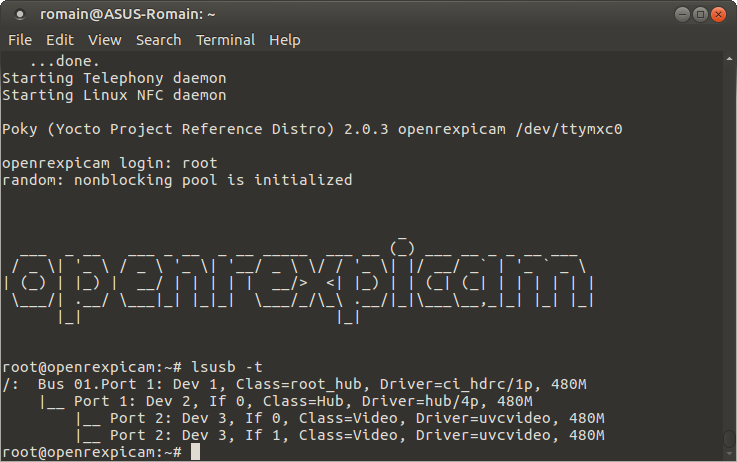
\includegraphics[width=1\linewidth,trim={0cm 0,6cm 0cm 12,5cm},clip]{webcam1.png}
    \decoRule
    \caption{Port USB de la webcam USB}  \label{fig:webcam1}   
\end{figure}

D’après la figure ci-dessus, nous en déduisons que la webcam USB est sur le bus
I2C n°1 et l’identifiant du port 1.2.

\begin{figure}[th]
    \centering
    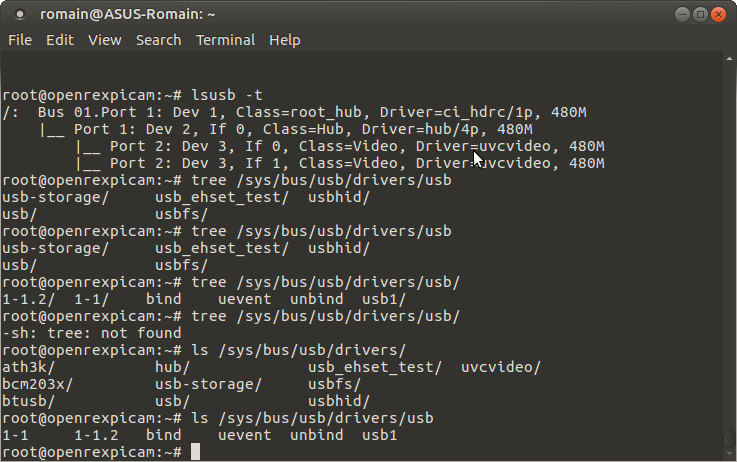
\includegraphics[width=1\linewidth,trim={0cm 0,6cm 0cm 14,5cm},clip]{webcam2.png}
    \decoRule
    \caption{Vérification du port et identifiant de la webcam USB}  \label{fig:webcam2}   
\end{figure}

Ensuite il faut écrire le numéro du bus et l’identifiant du port dans les fichiers
bind et unbind. Le fichier bind permette de  « lier » un appareil USB à son driver et
ainsi le rendre visible pour le système tandis que le fichier unbind lui détache le driver
de son appareil USB pour le « cacher » du système.

\begin{figure}[th]
    \centering
    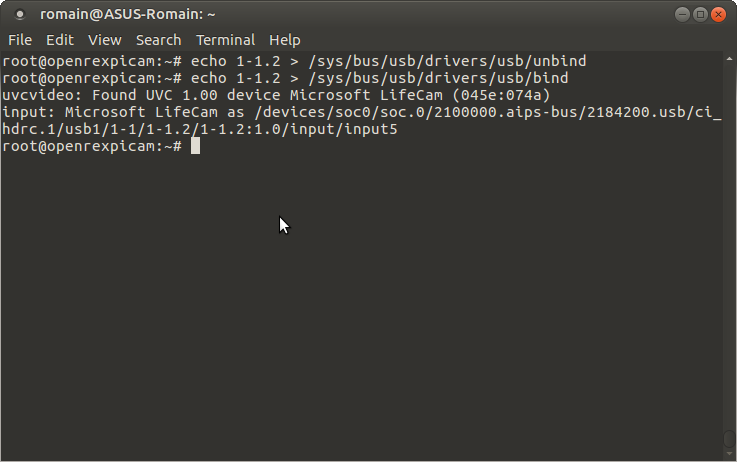
\includegraphics[scale=0.5,trim={0cm 11,5cm 0cm 1,7cm},clip]{webcam3.png}
    \decoRule
    \caption{Liaison entre la webcam USB et son driver}  \label{fig:webcam3}   
\end{figure}

On s’aperçoit bien que la webcam USB est bien reconnu par notre système puisquue
celui-ci nous affiche la référence de la webcam USB comme le montre l’illustration ci-dessus.

\begin{figure}[th]
    \centering
    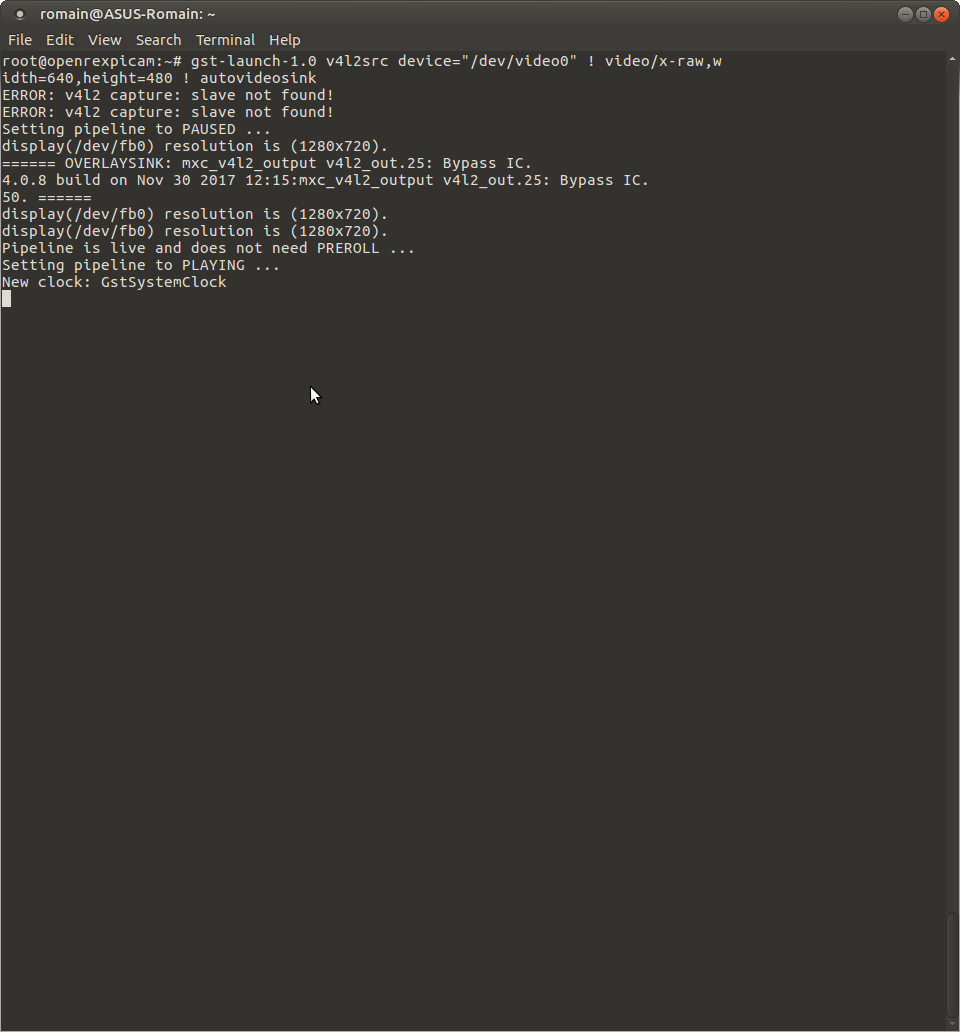
\includegraphics[scale=0.4,trim={0cm 26,1cm 0cm 1,7cm},clip]{webcam4.png}
    \decoRule
    \caption{Capture du flux vidéo de la webcam USB}  \label{fig:webcam4}   
\end{figure}

La commande \textbf{\# gst-launch-1.0 v4l2src device="/dev/video0" ! video/x-raw,w \\
idth=640,height=480 ! autovideosink} permet de démarrer un flux vidéo sur notre webcam USB.
Nous en sommes sûr puisque lorsque nous lançons la commande celle-ci se fige à « New clock :
GstSystemClock » , ça se fige exactement au même endroit que si nous effectuons cette commande
sur notre propre ordinateur et notre webcam intégré. De plus une petite LED verte s’allume
au moment de l’envoi de cette commande.

\begin{figure}[th]
    \centering
    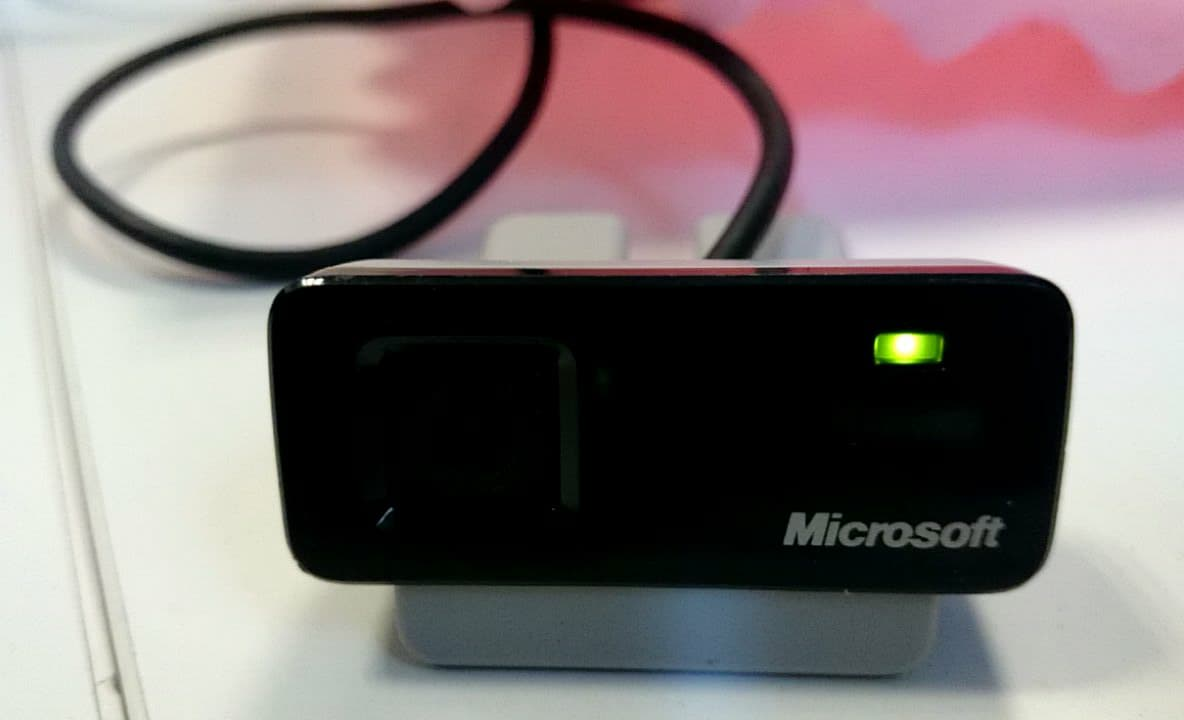
\includegraphics[scale=0.2,trim={10cm 2cm 4cm 9,5cm},clip]{webcam5.png}
    \decoRule
    \caption{LED verte allumée lors de l'envoi de la commande}  \label{fig:webcam5}   
\end{figure}

\section{Problèmes}

Notre principal problème pour l’instant est de récupérer ce flux vidéo puisqu’il
est impossible de l’afficher directement dans le terminal, pour tester cela nous
essayons de l’afficher sur nos ordinateurs par le réseau WiFi. 

\section{Point d'amélioration}

Dans un premier temps il est nécessaire de mettre l’image à jour pour que l’openrex
basic se connecte à un réseau WiFi, qui sera le même que nos ordinateurs, et dans un
second temps de récupérer ce flux vidéo par le réseau WiFi sur nos ordinateurs en UDP.


Finalement une fois que nous aurons réussi à afficher le flux vidéo de la webcam USB
sur nos ordinateurs nous essayerons d’effectuer le même processus mais pour la Raspi Cam v2,
qui est se pilote par le CSI et non l’USB.

\section{Sources}

\href{http://jas-hacks.blogspot.fr/2014/04/imx6-gstreamer-imx-and-usb-webcam.html}{http://jas-hacks.blogspot.fr/2014/04/imx6-gstreamer-imx-and-usb-webcam.html}